%% Source of figures/empirical-pipeline.pdf. Compile: pdflatex empirical-pipeline.tex
%% Generated 2026-10-28 from the SMOTE25 evaluation draft page (76 coded papers, 71 empirical).
%% Numbers are filled from the coded data; regenerate instead of editing them by hand.
\documentclass[tikz,border=4pt]{standalone}
\usepackage[scaled]{helvet}\renewcommand{\familydefault}{\sfdefault}
\usetikzlibrary{arrows.meta,positioning,fit}
\definecolor{sOne}{HTML}{2A78D6}\definecolor{sTwo}{HTML}{EB6834}\definecolor{sThree}{HTML}{1BAF7A}\definecolor{sFour}{HTML}{EDA100}
\definecolor{oZero}{HTML}{A3ABB4}\definecolor{oOne}{HTML}{5598E7}\definecolor{oTwo}{HTML}{1C5CAB}\definecolor{oThree}{HTML}{0D366B}\definecolor{inkTwo}{HTML}{465462}
\begin{document}
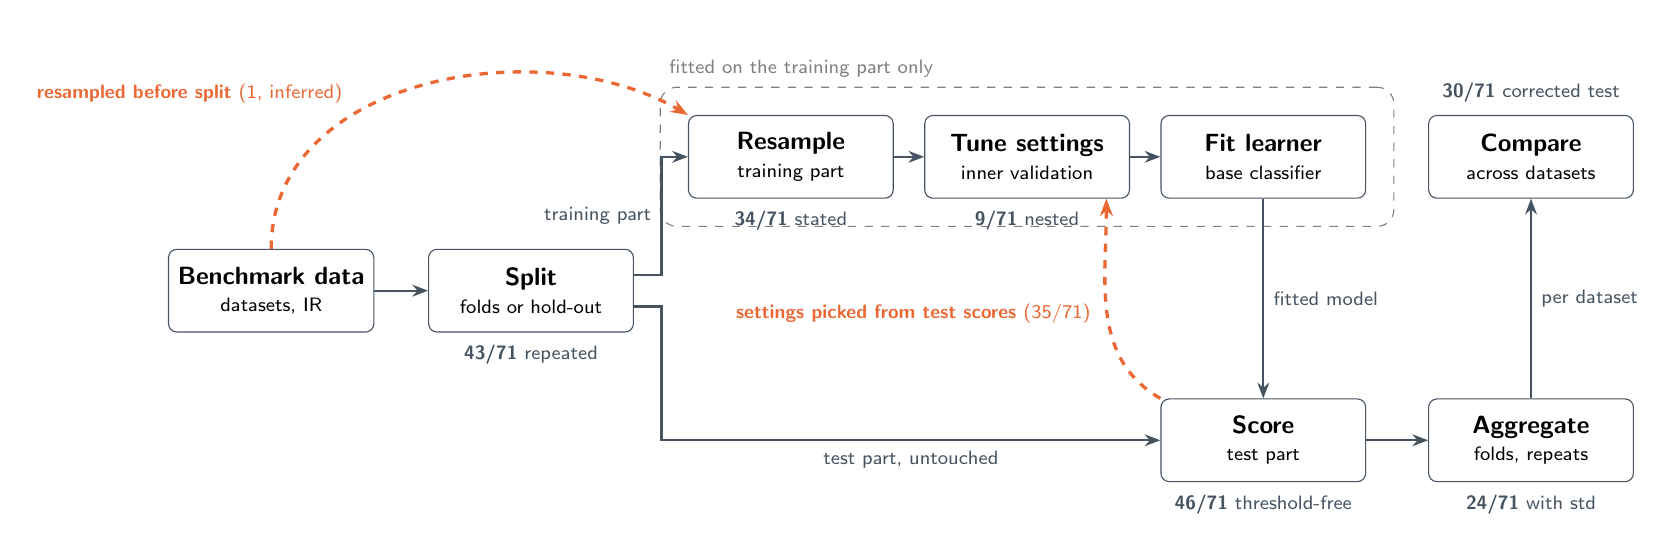
\begin{tikzpicture}[font=\small, box/.style={draw=inkTwo,rounded corners=3pt,minimum width=2.6cm,minimum height=1.05cm,align=center,fill=white}, stat/.style={font=\scriptsize,text=inkTwo}, flow/.style={-{Stealth[length=2mm]},draw=inkTwo,thick}, short/.style={-{Stealth[length=2.2mm]},draw=sTwo,very thick,dashed}, lab/.style={font=\scriptsize,text=inkTwo}]
\node[box] (data) at (0,0) {\textbf{Benchmark data}\\[-1pt]{\scriptsize datasets, IR}};
\node[box] (split) at (3.3,0) {\textbf{Split}\\[-1pt]{\scriptsize folds or hold-out}};
\node[box] (res) at (6.6,1.7) {\textbf{Resample}\\[-1pt]{\scriptsize training part}};
\node[box] (tune) at (9.6,1.7) {\textbf{Tune settings}\\[-1pt]{\scriptsize inner validation}};
\node[box] (fit) at (12.6,1.7) {\textbf{Fit learner}\\[-1pt]{\scriptsize base classifier}};
\node[box] (score) at (12.6,-1.9) {\textbf{Score}\\[-1pt]{\scriptsize test part}};
\node[box] (agg) at (16.0,-1.9) {\textbf{Aggregate}\\[-1pt]{\scriptsize folds, repeats}};
\node[box] (comp) at (16.0,1.7) {\textbf{Compare}\\[-1pt]{\scriptsize across datasets}};
\node[draw=gray,dashed,rounded corners=6pt,fit=(res)(tune)(fit),inner sep=10pt,label={[font=\scriptsize,text=gray,anchor=south west]north west:fitted on the training part only}] {};
\node[stat,below=1pt of split] {\textbf{43/71} repeated};
\node[stat,below=1pt of res] {\textbf{34/71} stated};
\node[stat,below=1pt of tune] {\textbf{9/71} nested};
\node[stat,below=1pt of score] {\textbf{46/71} threshold-free};
\node[stat,below=1pt of agg] {\textbf{24/71} with std};
\node[stat,above=1pt of comp] {\textbf{30/71} corrected test};
\draw[flow] (data) -- (split);
\draw[flow] ([yshift=2mm]split.east) -- ++(0.35,0) |- node[lab,pos=0.25,left] {training part} (res.west);
\draw[flow] (res) -- (tune);
\draw[flow] (tune) -- (fit);
\draw[flow] (fit) -- node[lab,right] {fitted model} (score);
\draw[flow] ([yshift=-2mm]split.east) -- ++(0.35,0) |- node[lab,pos=0.75,below] {test part, untouched} (score.west);
\draw[flow] (score) -- (agg);
\draw[flow] (agg) -- node[lab,right] {per dataset} (comp);
\draw[short] (data.north) to[out=90,in=150] node[lab,text=sTwo,pos=0.35,above left] {\textbf{resampled before split} (1, inferred)} (res.north west);
\draw[short] (score.north west) to[out=150,in=-90] node[lab,text=sTwo,pos=0.5,left=2pt] {\textbf{settings picked from test scores} (35/71)} ([xshift=-3mm]tune.south east);
\end{tikzpicture}
\end{document}
